\chapter{软件透明的一致性协议及其证明}
\label{chap:protocol}

本章描述ThyNVM双模式检查点生成技术使用的基于状态机的数据一致性协议,以及协议的形式化证明。

\section{地址空间管理}

ThyNVM使用两个地址转换表,\emph{块转换表}(BTT)和\emph{页转换表}(PTT),来维护从物理地址空间到硬件地址空间的映射。

每个物理地址在NVM上有一个对应的固定的\emph{主硬件地址}。所以,确定一个物理地址的主硬件地址不需要经过BTT或PTT进行地址转换。不失一般性,我们假定主硬件地址和物理地址相等。与此同时,任何物理地址都可以通过BTT或PTT被\emph{动态地}映射到一个NVM上的不同的硬件地址,映射方式取决于ThyNVM检查点生成模式的规则。

为了方便内存管理,我们将硬件地址空间划分为六个有不同用途的区域。图~\ref{fig:addr-space-detail}描绘了ThyNVM地址空间的组织形式。下面我们描述每个区域的用途。

\begin{figure}[!ht]
\centering
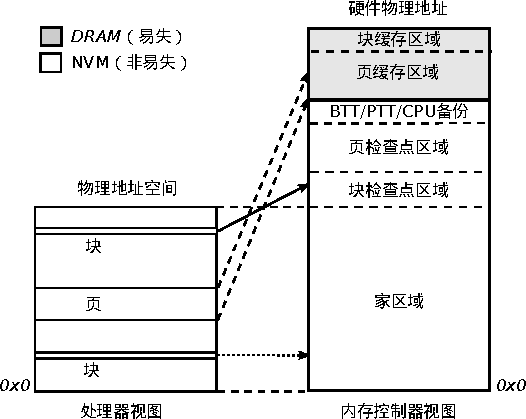
\includegraphics[width=0.7\linewidth]{addr-space-detail}
\caption{ThyNVM的物理和硬件地址空间。}
\label{fig:addr-space-detail}
\end{figure}


\textbf{家区域}:该区域位于NVM,包含所有主硬件地址。每个物理地址对应于一个本区域内的静态的主硬件地址。该区域的大小与物理地址空间的大小相同。

\textbf{块检查点区域}:该区域位于NVM,被BTT用来为检查点数据(\cl[block]或\cp[block])分配以缓存块大小为单位的存储空间。在块重映射模式中,一个块数据的工作副本(\wa[block])在其对应的BTT表项持久化后无需任何数据移动即可变为\cl[block]。所以,该区域同时保存着其BTT表项尚未持久化的\wa[block]数据。这样,一旦BTT完成持久化, 这些数据可以直接变成\cl[block]而不进行数据移动。

\textbf{页检查点区域}:该区域位于NVM,被PTT用来保存页粒度的检查点数据,即\cl[page]或\cp[page]。
家区域和页检查点区域交替保存\cl[page]和\cp[page]:如果\cp[page]保存在家区域中,那么\cl[page]则保存在本区域;反之亦然。

\textbf{页缓存区域}:该区域位于DRAM,是热点页工作副本(\wa[page])的缓存。在每个时间单元的检查点生成阶段,本区域中的脏页被回写到NVM作为\cl[page](位于上文描述的页检查点区域或家区域)。

\textbf{块缓存区域}:该区域位于DRAM,保存着一些块粒度的数据的临时副本。这些数据属于正在生成检查点的页。当程序执行和检查点生成过程重合时,对页缓存区域的写由块重映射模式处理,即被重映射到该区域做临时保存。

\textbf{BTT/PTT/CPU备份区域}:每个检查点生成阶段,BTT和PTT对应于{\cl}的版本都会保存在这个位于NVM中的区域。这样,当系统故障发生时,我们可以恢复出检查点数据所处的位置。检查点生成阶段开始时的CPU状态也保存在本区域,并与对应的BTT和PTT备份相关联。早于{\cp}版本的BTT/PTT/CPU备份可以被销毁。

这里的块检查点区域和页检查点区域共同对应于第\ref{subsec:thynvm-space}节描述的检查点区域A,而页缓存区域和块缓存区域则共同对应于工作数据区域。

\section{地址转换状态机}
\label{subsec:thynvm-state-machin}

我们使用一个状态机来决定一个内存写请求应当访问的位置,即将内存写请求的物理地址转换成一个合适的硬件地址。除了保存这个从物理地址到硬件地址的映射,每个BTT表项同时保存着7个状态之一,该状态驱动着块重映射模式的控制流。PTT重用与该状态机相同的逻辑,但只需要这些状态中的4个。下面我们聚焦于描述BTT的行为,而后讨论PTT如何适配到这个状态机的一个子集。图~\ref{fig-state-machine}描绘了状态机的全貌。为了清楚地展示,我们将状态分组而后逐组进行介绍。

\begin{figure}[!t]
\centering
\begin{tikzpicture}[->, >=stealth, node distance=0.37\tikzdistance, auto, thick,
font=\footnotesize, text centered]

\tikzstyle{every state}=[ellipse, inner sep=0pt]

\node[state] (h) [fill={rgb:black,1;white,4}] {\state{hidden}};
\node[state] (f) [right=of h, fill={rgb:black,1;white,4}] {\state{free}};
\node[state] (c) [above=of h, fill={rgb:black,1;white,4}] {\state{clean}};
\node[state] (t) [below left=of c] {\state{pre-hidden}};
\node[state] (d) [above=of f, fill={rgb:black,1;white,4}] {\state{dirty}};
\node[state] (s) [above right=of f] {\state{pre-dirty}};
\node[state] (l) [below right=of f] {\state{loan}};

\path (c.west)
  edge [bend right, anchor=south]
    node {\makecell[c]{write\\(ckpt.)\\\circled{$\mathnormal{6}$}}} (t);
\path (c)
  edge [anchor=east] node {\makecell[c]{write\\(exec.)\\\circled{$\mathnormal{3}$}}} (h)
  edge [anchor=west] node {\makecell[c]{revoke\\\circled{$\mathnormal{5}$}}} (f);
\path (h)
  edge [anchor=north] node {\makecell[c]{BTT flush\\\circled{$\mathnormal{4}$}}} (f)
  edge [loop, out=330, in=270, anchor=north, looseness=4]
    node [xshift=-0.05\tikzdistance] {write (exec.)} (h);
\path (t)
  edge [bend right, out=300, in=240, anchor=north]
    node [xshift=-0.1\tikzdistance] {\makecell[c]{write (exec.) $|$ clear\\\circled{$\mathnormal{7}$}}} (h)
  edge [loop, out=210, in=150, looseness=4, anchor=south]
    node [xshift=0.1\tikzdistance, yshift=0.15\tikzdistance]
      {\makecell[c]{write\\(ckpt.)}} (t);
\path (f)
  edge [anchor=west] node {\makecell[c]{write\\(exec.)\\\circled{$\mathnormal{1}$}}} (d)
  edge [bend right, anchor=base]
    node [xshift=0.12\tikzdistance, yshift=-0.05\tikzdistance] {\makecell[c]{\circled{$\mathnormal{8}$}\\write (ckpt.)}} (s)
  edge [bend right, anchor=base]
    node [xshift=-0.2\tikzdistance, yshift=-0.1\tikzdistance] {\makecell[c]{write'\\(ckpt.)}} (l);
\path (s)
  edge [bend right, anchor=west]
    node [xshift=-0.15\tikzdistance, yshift=0.05\tikzdistance]
      {\makecell[c]{write (exec.) $|$ clear\\\circled{$\mathnormal{9}$}}} (d)
  edge [loop, out=330, in=30, anchor=north, looseness=4]
    node [xshift=-0.12\tikzdistance, yshift=-0.1\tikzdistance]
      {\makecell[c]{write (ckpt.)}} (s);
\path (d)
  edge node [anchor=south] {\makecell[c]{BTT flush\\\circled{$\mathnormal{2}$}}} (c)
  edge [loop, out=60, in=120, looseness=4, anchor=south]
    node {write (exec.)} (d);
\path (l)
  edge [bend right, anchor=west]
    node {\makecell[c]{write' (exec.) $|$ clear \circled{$\mathnormal{10}$}}} (f)
  edge [loop, out=330, in=30, looseness=4, anchor=north]
    node [anchor=west] {\makecell[c]{write' (ckpt.)}} (l);

\end{tikzpicture}


\caption{在块重映射模式下,一个BTT表项的状态。每个内存写(“write”)后注明“exec.”或“ckpt.”,分别意味着该内存写到来的时间在程序执行阶段(无检查点生成)或在检查点生成阶段;“write'”指原本应到页缓存的写。}
\label{fig-state-machine}
\end{figure}

\subsection{执行时的状态}

该组状态主要协调模式在程序执行(没有检查点生成)时的行为。为了决定内存写的正确地址,我们需要一个状态记录关于地址映射的两方面信息:(1)该物理地址在当前活跃时间单元内是否被写过。如果是的话,我们可以直接覆写对应的硬件地址,因为同一个时间单元内对相同物理地址的内存写可以合并。(2)硬件地址是一个主硬件地址还是位于检查点区域中。在某些情况下,如果我们需要避免覆写其中一个的话,我们将选择另外一个。据此,我们有四个状态来涵盖上述两个选择的所有组合。

\begin{itemize}
\item \textbf{\state{Free}态}:标志一个空的无有效映射的表项。同时我们将没有包含在BTT中的物理地址默认为\state{free}态。这意味着其物理地址在当前活跃时间单元内没有被更改过,且其检查点数据位于家区域中的主硬件地址。新来的对该物理地址的写请求必须在BTT中开辟一个新的表项将这个写重映射到块检查点区域。

\item \textbf{\state{Clean}态}:该状态表明其物理地址在当前活跃时间单元没有被更改过,且其检查点数据位于块检查点区域。新来的对该物理地址的写请求必须被BTT重映射到家区域的主硬件地址以保护检查点数据。

\item \textbf{\state{Dirty}态}:该状态表明其物理地址在当前活跃时间单元内被更改过,且对应的硬件地址在块检查点区域。该映射可以继续有效直到当前时间单元结束,用以合并到相同物理地址的内存写。在当前时间单元结束后,该硬件地址上的数据应当变为检查点数据,所以这个表项会被备份到NVM,将映射关系持久化,以备系统故障时定位检查点数据。

\item \textbf{\state{Hidden}态}:这个状态表明其物理地址在当前活跃时间单元内被更改过,且对应的硬件地址是位于家区域的主硬件地址。这里实际上并没有地址转换,因为主硬件地址和物理地址是相等的。然而,该表项会一直存在直到当前时间单元结束,目的是合并同时间单元内对该物理地址的其他写。在当前时间单元结束后,这个表项会被清除。
\end{itemize}

\vspace{\noindentsep}
\noindent \textbf{实例  }为了展示上述状态之间的动态转换,我们构造了图~\ref{fig-example}中的实例。我们首先忽略检查点生成期间的步骤(步骤A和B),并简单假设它们没有发生。在这个实例中,我们展示了三个连续的时间单元,记为时间单元0到2。从时间单元$k$收到的内存写会产生数据版本$v_k$,其中$k = 0, 1, 2$。

\begin{figure}[!ht]
\centering
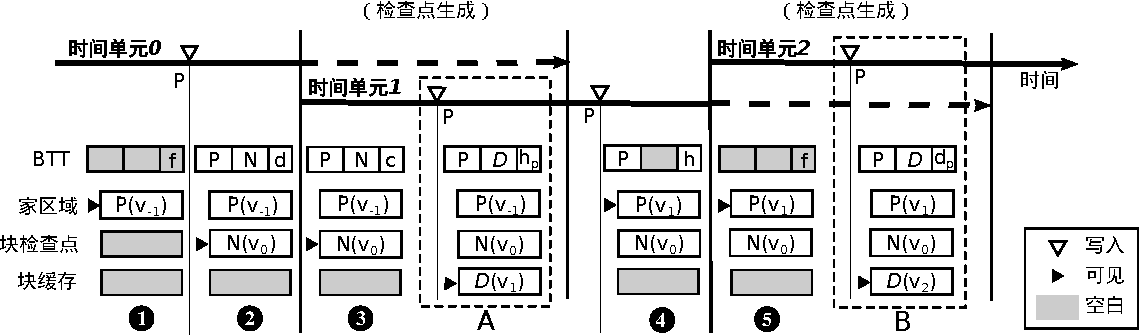
\includegraphics[width=\linewidth]{figures/example.pdf}
\caption{连续时间单元中对物理地址P进行多次内存写的实例。}
\label{fig-example}
\end{figure}

\vspace{\noindentsep}
\noindent\ding{202} 初始状态,我们假设在物理地址P的数据位于其主硬件地址(家区域),所以在BTT中没有对应的表项,且不占用块检查点区域或块缓存区域的位置。P位置的数据可以认为是最近检查点的版本(标记为$v_{-1}$,即$v_0$之前的一个版本)。

\vspace{\noindentsep}
\noindent\ding{203} 在执行时间单元0的过程中,当一个对物理地址P的内存写到达时,我们不能覆写家区域中的检查点数据$v_{-1}$。所以,一个新的映射P-N被添加到BTT中,将数据$v_0$导向块检查点区域中的硬件地址N。我们将该表项标记为\state{dirty}态(图~\ref{fig-state-machine}中的状态转换\circled{$\mathnormal{1}$})以表明该物理地址在当前活跃时间单元内已经被更改过。这个时间单元内后续的任意对物理地址P的内存写都可以合并在硬件地址N。

\vspace{\noindentsep}
\noindent\ding{204} 在时间单元0之后,上述\state{dirty}表项被冲刷到BTT/PTT/CPU备份区域。该表项在BTT中的状态变为\state{clean}(状态转换\circled{$\mathnormal{2}$})以表明该映射已经持久化且在新的时间单元1中尚无对该物理地址的写。

\vspace{\noindentsep}
\noindent\ding{205} 时间单元0完成检查点生成之后,我们不再需要家区域中的数据$v_{-1}$。所以对物理地址P的内存写可以直接映射到主硬件地址。与此同时,相应的BTT表项状态变为\state{hidden}态(状态转换\circled{$\mathnormal{3}$})。该状态表明主硬件地址保存着数据$v_1$,而且这个时间单元内对P的后续写可以在这个位置上更新数据。如果这一步出现系统故障,ThyNVM则会回退到块重映射区域保存的数据$v_{0}$。

\vspace{\noindentsep}
\noindent\ding{206} 当时间单元2开始时,BTT冲刷操作已经将\state{hidden}状态清除,而这个表项被释放以表明家区域中的主硬件地址保存着物理地址P的数据的最近检查点版本$v_1$(状态转换\circled{$\mathnormal{4}$})。

我们可以看到,该BTT表项在连续多个时间单元收到内存写之后会变为\state{free}态。所以,多个时间单元之间的时间局部性可以减少使用中的表项,进而缓解对有限的BTT的存储空间的压力。在最坏状态下,如果BTT没有\state{free}状态的表项,我们必须撤销一个\state{hidden}态或者\state{clean}态的表项为新的内存写提供空间。\state{Hidden}态的表项无论如何都会在当前活跃时间单元结束时被撤销;
\state{Clean}态的表项可以被安全撤销(状态转换\circled{$\mathnormal{5}$})是因为他们不记录当前活跃时间单元内的新的更新。然而,被\state{clean}态表项引用的数据块(位于块检查点区域)需要和其主硬件地址上的数据互换。

\subsection{检查点生成时的状态}
\label{subsec:states-ckpt}

第二个状态组在检查点生成阶段发挥作用。该组包含两个状态,\state{pre-hidden}态和\state{pre-dirty}态,分别处理如下两种情况。

\begin{itemize}
\item
\textbf{\state{Pre-hidden}}态:该状态处理一个\state{clean}态的物理地址在检查点生成阶段收到内存写的情况。我们不能简单地像程序执行阶段一样执行状态转换\circled{$\mathnormal{3}$},因为家区域和块检查点区域的数据在检查点生成阶段都必须被保留。以图~\ref{fig-example}中的步骤A为例。因为我们当前处于时间单元1,块检查点区域的数据$v_0$是不可更改的,因为它是最近检查点 \cl 的一部分;同样地,家区域中的数据$v_{-1}$也不可更改,因为完整的一致的 \cl 尚未完成——如果此时系统故障终断了检查点生成进程,系统会回滚到$v_{-1}$(即 \cp)。因此,我们需要临时将工作数据(\wa)放入另外一个地方,块缓存区域,并相应地把这个特别的状态标记为\state{pre-hidden}(状态转换\circled{$\mathnormal{6}$})。\state{Pre-hidden}状态是\state{clean}状态和\state{hidden}状态之间的一个垫脚石。它只在当前活跃时间单元结束前存在。之后,如果该状态没有被一个内存写驱动转换到\state{hidden}(达到图~\ref{fig-example}中步骤4相同的结果),它会被显式地清理(状态转换\circled{$\mathnormal{7}$})。不论哪种情况,因为时间单元0的检查点(\cl)已经完成,版本$v_{-1}$(\cp)都会被工作数据 \wa 安全地覆写,并相应收回块缓存区域里 \wa 的位置。
\item
\textbf{\state{Pre-dirty}}态:该状态处理一个\state{free}态的物理地址在检查点生成阶段收到内存写的情况。与\state{pre-hidden}的处理逻辑类似,我们不能像程序执行阶段一样直接执行状态转换\circled{$\mathnormal{1}$}。以图~\ref{fig-example}中的步骤B为例。当时间单元1的检查点(\cl)正在生成的时候,我们不仅要保留$v_1$,还要保留$v_0$(\cp),因为 \cp 是我们仅有的完整一致的检查点。所以,我们把数据$v_2$放入块缓存区域,并向BTT添加一个\state{pre-dirty}态的表项来记录该映射(状态转换\circled{$\mathnormal{8}$})。\state{Pre-dirty}状态或者被下一个程序执行阶段的内存写命中转换到\state{dirty}态,或者在那个阶段结束时被清理转换到\state{dirty}态(状态转换\circled{$\mathnormal{9}$})。
\end{itemize}

因为\state{hidden}态和\state{dirty}态在每个检查点生成阶段刚刚开始时伴随BTT冲刷操作被清理,他们永远不会在检查点生成阶段与内存写相遇。所以,我们没有其他情况需要处理。

\subsection{用于双模式合作的状态}

最后我们有一个用于两个模式间合作的状态。当页回写模式生成脏页的检查点时,对这些页的各个内存写暂由块重映射模式重定向到块缓存区域(与第\ref{subsec:states-ckpt}节介绍的操作类似)。我们不把这些BTT表项混入上文的那些状态和转换,所以这些表项被标记为\state{loan}。当检查点生成结束这些页面重新可以被直接修改的时候,\state{Loan}态的表项最终将数据移回原页中(状态转换\circled{$\mathnormal{10}$})。

\section{正确性定义}

本节给出一致性协议正确性证明的定义。我们这里聚焦于ThyNVM检查点生成模式的故障时一致性,亦即可恢复性——任何时候系统发生故障,ThyNVM可以恢复最近的一致的检查点。特别地,假设$t_k$为时间单元$k$结束执行的时刻,那么在$t_{k-1}$和$t_k$之间,ThyNVM顺次经历两个时间阶段,即一个检查点生成阶段(与时间单元$k+1$的程序执行阶段重合)和一个程序执行阶段(指没有与检查点生成重合的部分);$t_k$时刻的数据快照记为版本$v_k$,亦即时间单元$k$的检查点版本。我们将证明如下两个不变式,在状态机的转换中一直保持成立。

\begin{enumerate}
\item \label{invar-ckpt} 在时刻$t_{k-1}$与$t_k$之间的检查点生成阶段,数据版本$v_{k-1}$和$v_{k-2}$及其在地址转换表中的映射都被保留。
\item \label{invar-exec} 在时刻$t_{k-1}$与$t_k$之间的程序执行阶段,数据版本$v_{k-1}$及其在地址转换表中的映射都被保留。
\end{enumerate}

显然,如果上述两个不变式成立,那么系统在检查点生成阶段或程序执行阶段发生故障时,可以分别恢复到{\cp}或{\cl}。

\section{块重映射模式的正确性证明}

ThyNVM的块重映射模式由第\ref{subsec:thynvm-state-machin}节的状态机描述。对于任何由状态机转换形成的状态序列,我们使用数学归纳法\cite{Hopcroft:ALC:2006}验证上节两个不变式的正确性。

\subsection{数据抽象}

为了实施形式化证明,我们使用变量来代表ThyNVM中的数据结构,如图\ref{fig-data-struct}所示。由于我们只关心数据版本而非具体的数据,不妨认为这些变量保存着数据版本值;大写的变量值表示集合。因为所有 BTT表项互斥,我们仅关心任意一个BTT表项,并假设该表项当前是用于物理地址\phy{P}。

\begin{figure}[!t]
\centering
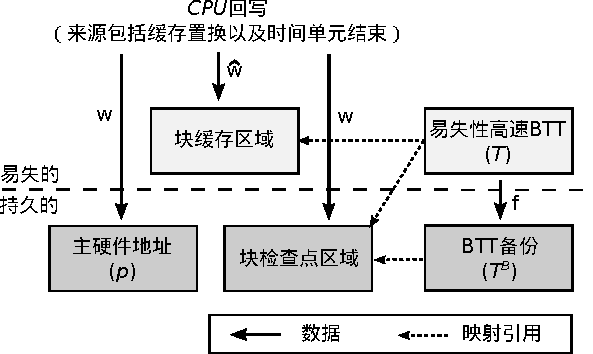
\includegraphics[width=0.9\columnwidth]{data-struct}
\caption{ThyNVM中的数据结构及其符号。}
\label{fig-data-struct}
\end{figure}

\begin{itemize}
\item $p$ 保存着主硬件地址\nvm{P}上的数据块的版本号。
\item $T$ 保存着对应于\phy{P}的BTT表项。该表项是易失的。如果没有对应于\phy{P}的BTT表项,那么
$T=\varnothing$,此时可认为\phy{P}的状态为\state{free};否则,我们恒有$\left\vert{T}\right\vert = 1$,其中唯一的项保存着在块检查点区域中对应数据块的版本号。
\item $T^B$ 保存着持久化的BTT表项,位于BTT备份区域。类似地,我们有$\left\vert{T^B}\right\vert \le 1$。特别地,对于时间单元$0$,我们仅出于方便计算的目的认为$T^B \subset \{-1, -2\}$。
\end{itemize}

另外,下面的字母代BTT表项状态机的输入。

\begin{itemize}
\item $\mathbf{w}$和$\mathbf{\hat{w}}$分别表示在程序执行阶段和检查点生成阶段向物理地址\phy{P}的写操作。
\item $\mathbf{r}$和$\mathbf{\hat{r}}$分别表示在程序执行阶段和检查点生成阶段撤销物理地址\phy{P}对应的BTT表项。
\item $\mathbf{f}$表示刷出BTT到备份区域。该事件标志一个检查点阶段的开始。
\item $\mathbf{c}$表示在刷出BTT之前清理\state{pre-dirty}态和\state{pre-dirty}态表项的操作。
\end{itemize}

\subsection{行为抽象}

基于如上的变量和符号,我们将主要的状态转换过程表述为过程\ref{alg-dirty}到\ref{alg-free-c}。相应地,BTT表项的状态机也可改写为图\ref{fig:asm}。注意\state{loan}态没有在图中画出,而是在第\ref{sec:proof-page-writeback}节单独讨论。

\begin{algorithm} [!h]
\caption{转换至\state{dirty}态}
\label{alg-dirty}
\begin{algorithmic}[1]
\Require 处于程序执行阶段。
\State 在块检查点区域分配地址\nvm{N}
\State 将数据块$v_0$写入\nvm{N}
\If{表项是\state{pre-dirty}态,即映射关系为\phy{P}-\dram{D}}
  \State 从块缓存区域撤销位于\dram{D}的数据块
\EndIf
\State 设置表项为\state{dirty}态,即映射关系为\phy{P}-\nvm{N} \Comment{$T \leftarrow \{0\}$}
\end{algorithmic}
\end{algorithm}

\begin{algorithm} [!h]
\caption{临时缓存数据块}
\label{alg-hold}
\begin{algorithmic}[1]
\Require 处于检查点生成阶段。
\State 在块缓存区域分配地址\dram{D}
\State 将数据块$v_0$写入\dram{D}
\If{表项是\state{clean}态,即映射关系为\phy{P}-\nvm{N}}
  \State 将位于\nvm{N}的数据标记为在下一个检查点生成阶段被撤销
  \State 将表项转换至\state{pre-hidden}态
\ElsIf{表项是\state{free}态}
  \State 将表项转换至\state{pre-dirty}态
\EndIf
\State 设置映射关系为\phy{P}-\dram{D} \Comment{$T \leftarrow \{0\}$}
\end{algorithmic}
\end{algorithm}

\begin{algorithm} [!h]
\caption{转换至\state{hidden}态}
\label{alg-hide}
\begin{algorithmic}[1]
\Require 处于程序执行阶段。
\State 将数据块$v_0$写入主硬件地址 \Comment{$p \leftarrow 0$}
\If{表项是\state{clean}态,即映射关系为\phy{P}-\nvm{N}}
  \State 将位于\nvm{N}的数据标记为在下一个检查点生成阶段被撤销
\ElsIf{表项是\state{pre-hidden}态,即映射关系为\phy{P}-\dram{D}}
  \State 从块缓存区域撤销位于\dram{D}的数据块
\EndIf
\State 将表项转换至\state{hidden}态 \Comment{$T \leftarrow \{p\}$}
\end{algorithmic}
\end{algorithm}

\begin{algorithm} [!h]
\caption{撤销\state{clean}态的映射关系\phy{P}-\nvm{N}}
\label{alg-free-c}
\begin{algorithmic}[1]
\If{处于程序执行阶段}
  \State 将位于\nvm{N}的数据块$v_{-1}$写入\nvm{P},覆盖数据块$v_{-2}$ \Comment{$p \leftarrow -1$}
  \State 将位于\nvm{N}的数据标记为在下一个检查点生成阶段被撤销
\Else \Comment{处于检查点生成阶段}
  \State 交换位于\nvm{P}的数据块$v_{-2}$和位于\nvm{N}的数据块$v_{-1}$ \Comment{$T^B \leftarrow (T^B - T) \cup \{p\}$}
  \Statex \Comment{$p \leftarrow -1$}
  \State 在BTT备份(对应于$v_{-1}$)中标记\phy{P}-\nvm{N}为已置换
  \State 将位于\nvm{N}的数据块标记为在下一个检查点生成阶段被撤销
\EndIf
\State 将表项转换至\state{free}态,即撤销该表项 \Comment{$T \leftarrow \{p\}$}
\end{algorithmic}
\end{algorithm}

\begin{figure}[!t]
\centering
\begin{tikzpicture}[->, >=stealth, node distance=0.38\tikzdistance, auto, thick,
font=\footnotesize]

\tikzstyle{every state}=[ellipse, inner sep=1pt]

\node[state] (h) {\state{hidden}};
\node[state] (f) [right=of h] {\state{free}};
\node[state] (c) [above=of h] {\state{clean}};
\node[state] (t) [below left=of c] {\state{pre-hidden}};
\node[state] (d) [above=of f] {\state{dirty}};
\node[state] (s) [above right=of f] {\state{pre-dirty}};

\path (c.west)
  edge [bend right, anchor=south]
    node [xshift=-0.18\tikzdistance]
      {\trans{\mathbf{\hat{w}}}{Procedure~\ref{alg-hold}}} (t);
\path (c)
  edge [bend right, anchor=base]
    node {\trans{\mathbf{w}}{Procedure~\ref{alg-hide}}} (h)
  edge [anchor=base] node {\trans{\mathbf{r, \hat{r}}}{Procedure~\ref{alg-free-c}}} (f);
\path (h)
  edge [anchor=south] node {$\mathbf{f}$} (f)
  edge [loop, out=330, in=270, anchor=north, looseness=4]
    node {$\mathbf{w}$} (h);
\path (t)
  edge [bend right, out=300, in=240, anchor=north]
    node {\trans{\mathbf{w, c}}{Procedure~\ref{alg-hide}}} (h)
  edge [loop, out=210, in=150, looseness=4, anchor=south]
    node [xshift=0.1\tikzdistance, yshift=0.15\tikzdistance]
      {$\mathbf{\hat{w}}$} (t);
\path (f)
  edge [bend right, anchor=base]
    node {\trans{\mathbf{w}}{Procedure~\ref{alg-dirty}}} (d)
  edge [bend right, anchor=west]
    node {\trans{\mathbf{\hat{w}}}{Procedure~\ref{alg-hold}}} (s);
\path (s)
  edge [bend right, anchor=south]
    node [xshift=0.15\tikzdistance]
      {\trans{\mathbf{w, c}}{Procedure~\ref{alg-dirty}}} (d)
  edge [loop, out=330, in=30, anchor=south, looseness=4]
    node [xshift=-0.12\tikzdistance, yshift=0.15\tikzdistance]
      {$\mathbf{\hat{w}}$} (s);
\path (d)
  edge node [anchor=south] {$\mathbf{f}$} (c)
  edge [loop, out=60, in=120, looseness=4, anchor=south]
    node {$\mathbf{w}$} (d);

\end{tikzpicture}


\caption{State machine of BTT entry for THNVM block remapping scheme.}
\label{fig:asm}
\end{figure}

\subsection{证明步骤}

每一个输入的写操作驱动状态机进行一步转换。 因此,我们可以为所有变量添加一个下标$n$,以标示变量值对应于状态机状态转换序列中的哪一步。我们采用数学归纳法的证明基于$n$进行推导。

\textbf{命题}:不变式~\ref{invar-exec}和不变式~\ref{invar-ckpt}可以分别翻译为如下两个命题$P(n)$和$Q(n)$。

在程序执行阶段,我们需要保证$P(n)$一直成立:$$ P(n)=(-1 \in T^B_n) \vee (-1 \notin T^B_n \wedge p_n=-1). $$ 我们假设当前活跃时间单元为0。上式隐含了两个可以接受的情况。第一个是BTT备份包含一个指向块检查点区域的映射(即$-1 \in T^B_n$)。第二个是BTT备份不包含对$v_{-1}$的映射关系(即$-1 \notin T^B_n$)但{\cl}处于主硬件地址(即$p_n=-1$)。只要两个情况任一成立,那么系统故障发生时,从BTT备份中恢复出BTT可使ThyNVM找到地址\phy{P}的正确的{\cl},即$v_{-1}$。

在检查点生成阶段,我们需要保证$Q(n)$一直成立:$$ Q(n)=(p_n=-2 \wedge -1 \in T^B_n) \vee (p_n=-1 \wedge -2 \in T^B_n). $$ 与$P(n)$类似,$Q(n)$意味着两个正确的情况:BTT备份包含{\cl}($v_{-1}$)的映射并指向块检查点区域(即$-1 \in T^B_n$),而\cp($v_{-2}$)位于主硬件地址,依然得到保留(即$p_n=-2$);或者两个版本所处位置相反的情况——如果主硬件地址保存着{\cl},那么BTT备份必须记录着{\cp}的位置(即$p_n=-1 \wedge -2 \in T^B_n$)。

综上,我们需要证明如下这个命题:$$S(n)=(\alpha_n \in
\{\mathbf{w}, \mathbf{r}, \mathbf{c}\} \wedge P(n)) \vee (\alpha_n \in
\{\mathbf{\hat{w}}, \mathbf{\hat{r}}, \mathbf{f}\} \wedge Q(n))$$
我们通过区分输入的字母$\alpha_n$来判断处于程序执行阶段还是检查点生成阶段。 $\mathbf{w}、\mathbf{r}$和$\mathbf{c}$在程序执行阶段输入,而其余的在检查点生成阶段出现。

\textbf{归纳基础}:
在整个系统最初始的状态,我们可以认为所有数据均位于主硬件地址。不妨假设初始步骤前存在虚拟的时间单元-1,那么有$p_0=-1$;另外,由于BTT为空,我们有$T^B_0=\varnothing$。所以,$P(0)$成立。进而,由于处在程序执行阶段,$S(0)$是成立的,值为真。

\noindent\textbf{归纳步骤}:
假设对任意的$n \ge 1$,$S(n-1)$为真,下面我们论证$S(n)$也为真。

首先,我们统一考虑状态机中所有自循环。对于状态\state{dirty}、\state{pre-dirty}和\state{pre-hidden},ThyNVM只更新$T_n$,所以$S_n=S_{n-1}$为真。对于状态\state{hidden},ThyNVM令$p_n=0$,但根据将状态转换至\state{hidden}的过程\ref{alg-hide},在自循环前即有$p_{n-1}=0$,所以ThyNVM并没有更改该值。所以我们也可以得到$S_n=S_{n-1}$。

其次,我们看两个包含BTT冲刷$\mathbf{f}$的状态转换。

$\state{dirty} \rightarrow \state{clean}$:转换前的状态为\state{dirty}表明$p_{n-1}=-1$。转换后,新的时间单元与检查点生成阶段重合,所以我们有$p_n=-2$\footnote{只有BTT刷出操作会将所有的版本号减一。任何其他过程中,版本号或者保持或者被显式赋值}。另外,ThyNVM将\state{clean}态的映射写入BTT备份,意味着$-1$被加入$T^B_n$。所以,我们有$p_n=-2 \wedge -1 \in T^B_n$,也就是$Q(n)$成立。进而,$S(n)$为真。

$\state{hidden} \rightarrow \state{free}$:转换前的状态是\state{hidden}意味着$p_{n-1}=0$,而在程序执行阶段,$S(n-1) \implies P(n-1)$,所以$-1 \in T^B_{n-1}$必为真。状态转换之后,由于处在新的时间单元,我们有$p_n=-1$以及$-2 \in T^B_n$。所以$Q(n)$为真,进而$S(n)$成立。

除去上述情况,步骤$n$必然经历下面的过程。

过程\ref{alg-dirty}管理着状态转换$\state{free} \rightarrow
\state{dirty}$和$\state{pre-dirty} \rightarrow \state{dirty}$。不论哪个状态转换,该过程保护$p=-1 \wedge -1 \notin T^B$:转换前,状态\state{free}和\state{pre-dirty}都有$p_{n-1}=-1 \wedge -1 \notin
T^B_{n-1}$,而该过程避免覆写主硬件地址,所以我们有$p_n=-1$。而且,该过程不刷出表项到BTT备份区域,所以有$-1 \notin T^B_n$。因此,$P(n)$成立。又因为处在程序执行阶段(即$\alpha_n \in \{\mathbf{w}, \mathbf{r}, \mathbf{c}\}$),我们有$S(n-1) \implies S(n)$。

过程\ref{alg-hold}管理着状态转换$\state{clean} \rightarrow
\state{pre-hidden}$和$\state{free} \rightarrow \state{pre-dirty}$。不论哪个状态转换,该过程将数据写入块缓存区域,而不是更改$p$或$T^B$。这么做的目的是在检查点生成阶段保护$v_{-1}$和$v_{-2}$。因此,不难得出$S(n)=S(n-1)$。

过程\ref{alg-hide}管理着状态转换$\state{clean} \rightarrow
\state{hidden}$和$\state{pre-hidden} \rightarrow \state{hidden}$。转换前,状态\state{clean} 和\state{pre-hidden}必然处在检查点生成阶段,所以有$p_{n-1}=-2 \wedge -1 \in T^B_{n-1}$ (根据BTT刷出行为和过程\ref{alg-hold})。在该过程中,ThyNVM设置$p_n=0$但不涉及$T^B$,所以我们有$p_n=0 \wedge -1 \in T^B_n$。又因为处于程序执行阶段,$S(n)$为真。

过程\ref{alg-free-c}管理着状态转换$\state{clean} \rightarrow \state{free}$,但有可能处于程序执行阶段,也可能处于检查点生成阶段。状态转换器前,依据BTT刷出行为我们有
$P_{n-1}=-2 \wedge -1 \in T^B_{n-1}$,且被$T$引用的最近的版本是$v_{-1}$。如果处于程序执行阶段,该过程设置
$p_n=-1$,但保持$-1 \in T^B_n$,所以$P(n)$成立。进而,$S(n)$为真。如果处于检查点生成阶段,ThyNVM交换$p$和$T^B$的值,从而导致
$p_n=-1 \wedge -2 \in T^B_n$。相应地,$Q(n)$成立,且$S(n)$为真。

综上,对于状态机在所有可能的转换中所遵循的路径,恒有$S(n-1)
\implies S(n)$。考虑到初始步骤0符合$S(0)$,我们可以得出结论$S(n)$对所有的$n \ge 0$成立。也就是说,不变式\ref{invar-ckpt}和\ref{invar-exec}对任何物理地址均成立。


%Finally, we explain why the number of \textsc{Block Buffer} slots should be twice
%the number of BTT entries, even though any particular physical address only
%requires up to one slot in \textsc{Block Buffer} as shown above. Apparently, we
%have $\left\vert{T^B}\right\vert \le 1$ for any single physical address served
%by BTT, and it references up to one \textsc{Block Buffer} slot. However, when
%there is a \state{free} BTT entry, it may serve a different physical address
%upon request. This does not affect consistency or recoverability of either
%address, but requires extra \textsc{Block Buffer} slots as the new address may
%need a second \textsc{Block Buffer} slot. For example, suppose a BTT entry for
%\phy{P} shifts from \state{clean} to \state{free} in an execution phase, then we
%have $-1 \in T^B$ and it references a \textsc{Block Buffer} slot. Afterwards, if we
%receive a write to another physical address \phy{P'}, we may have to set up a
%\state{dirty} mapping for \phy{P'} using this \state{free} entry. In that case, $T$ maps
%to a second slot in \textsc{Block Buffer}.
%
%Meanwhile, no matter how many physical addresses the BTT serves, we have at most
%two versions of full BTT in \textsc{BTT Backup}, so they reference \textsc{Block
%Buffer} slots of at most twice the number of BTT entries. Further, when
%\textsc{Block Buffer} slots are occupied by previous versions of data ($v_{-1}$
%and $v_{-2}$ referenced by \textsc{BTT Backup}), the current version of data
%($v_0$) will locate in \textsc{Block Cache} via \state{pre-hidden} and
%\state{pre-dirty}.

\section{页回写模式的正确性证明}
\label{sec:proof-page-writeback}

为了简便,我们在证明中忽略不重要的部分。首先,我们认为如下\emph{独立的回写模式}的正确性自明:(1)在检查点生成阶段停止一切对内存的修改;(2)将缓存的脏页写入NVM作为检查点,但是不覆写它们之前的版本;(3)原子性地将记录所有检查点页位置的表写入NVM。显然,不变式\ref{invar-ckpt}和\ref{invar-exec}都是成立的。 

对于上述步骤(2),我们重用块重映射模式的状态机来维护故障时数据一致性。特别地,我们只需做如下替换:第一,块重映射协议中的程序执行阶段和检查点生成阶段在这个过程中都被认为是程序执行阶段,所以只有\state{free}、
\state{dirty}、\state{clean}和\state{hidden}四个状态有效。第二,块检查点区域由页检查点区域代替。第三,所有写变为页粒度,而不再是块粒度。因此,这个过程可以视作之前论证的重映射模式的一个特例,其正确性可以得到保证。

进而,基于上述独立的回写模式的正确性,我们可以得出ThyNVM采用的页回写模式的正确性。当生成脏页的检查点时,块重映射模式会临时负责代理应用程序写往页缓存区域的新的请求,所以ThyNVM的页回写模式与独立的页回写模式等价,当且仅当满足如下两个条件:(1)页缓存区域保存着在生成检查点开始前保存着数据的最新的一致的版本;(2)页缓存区域的这一状态在整个检查点生成阶段得以保持。

第一个条件可以满足,因为在程序执行阶段页缓存区域是直接更新的,而保存在块缓存区域中的数据会在检查点生成阶段前移回页缓存区域(由一个清理操作完成)。第二个条件也成立,因为在检查点生成阶段,应用程序的新的写都被转移到块缓存区域而不会污染页缓存区域。综上,ThyNVM的页回写模式被证明是正确的。
